%!TEX TS-program = xelatex
%!TEX encoding = UTF-8 Unicode

\documentclass[12pt,a4paper]{article}
\usepackage{fontspec,xltxtra,xunicode}
\usepackage{fancyhdr}
\usepackage[a4paper,margin=3cm]{geometry}
\setmainfont[Scale=1.22]{TH Sarabun New}
\XeTeXlinebreaklocale 'th_TH'

% Source code
\usepackage{listings}
\lstdefinestyle{sitdhcodelisting}{
    frame=trBL,
    label=trianglecheck,
    showspaces=false,
    numberstyle=\tiny, 
    language=Java, 
    numbers=left,   
    firstline=1
}

% Graphic
\usepackage{graphicx}
% Multiple row
\usepackage{multirow}
% Table
\usepackage{array}
% Landscape page
\usepackage{pdflscape}

\newcommand{\sitdhibong}{สิทธิพงษ์ เหล่าโก้ก}
\newcommand{\studentid}{5870972621}
\newcommand{\department}{สาขาวิชาวิศวกรรมซอฟต์แวร์}
\newcommand{\faculty}{คณะวิศวกรรมศาสตร์}
\newcommand{\myprogram}{แผน ข. ภาคนอกเวลาราชการ}
\newcommand{\university}{จุฬาลงกรณ์มหาวิทยาลัย}
\newcommand{\subject}{Software Testing and Quality Assurance}
\newcommand{\outbound}{Some input value is out of range}
\newcommand{\nottriangle}{Not a triangle}
\newcommand{\equ}{Equilateral}
\newcommand{\sca}{Scalene}
\newcommand{\iso}{Isoscalene}

\renewcommand{\lstlistingname}{รายการที่}
\renewcommand{\figurename}{ภาพที่}
\renewcommand{\tablename}{ตารางที่}

\pagestyle{fancy}
\lhead{\subject}
\rhead{การบ้านครั้งที่ 4: Path testing}
\lfoot{\sitdhibong: \studentid}

% Source code cosmatic
\lstset{columns=fullflexible,basicstyle=\ttfamily}

\begin{document}
% Triangle check
\section{โปรแกรมคำนวณรูปสามเหลี่ยม}
\label{listing:trianglecal}
จากรายการความต้องการเพื่อตรวจสอบรูปสามเหลี่ยม จะนำมาเขียนโปรแกรมด้วยภาษา JavaScript ดังแสดงให้เห็นด้านล่าง
\lstinputlisting[style=sitdhcodelisting, title=\lstname, caption=โปรแกรมตรวจสอบรูปสามเหลี่ยมภาษา JavaScript]{src/compute.js}

\newpage
% Control flow graph
\section{Control flow graph}
จากโปรแกรมคำนวณรูปสามเหลี่ยมจาก \lstlistingname\, \ref{listing:trianglecal} นำมาวาด Control flow graph ได้ดังรูปด้านล่าง

\begin{figure}[h!]
    \label{fig:flowgraph}
    \centering
    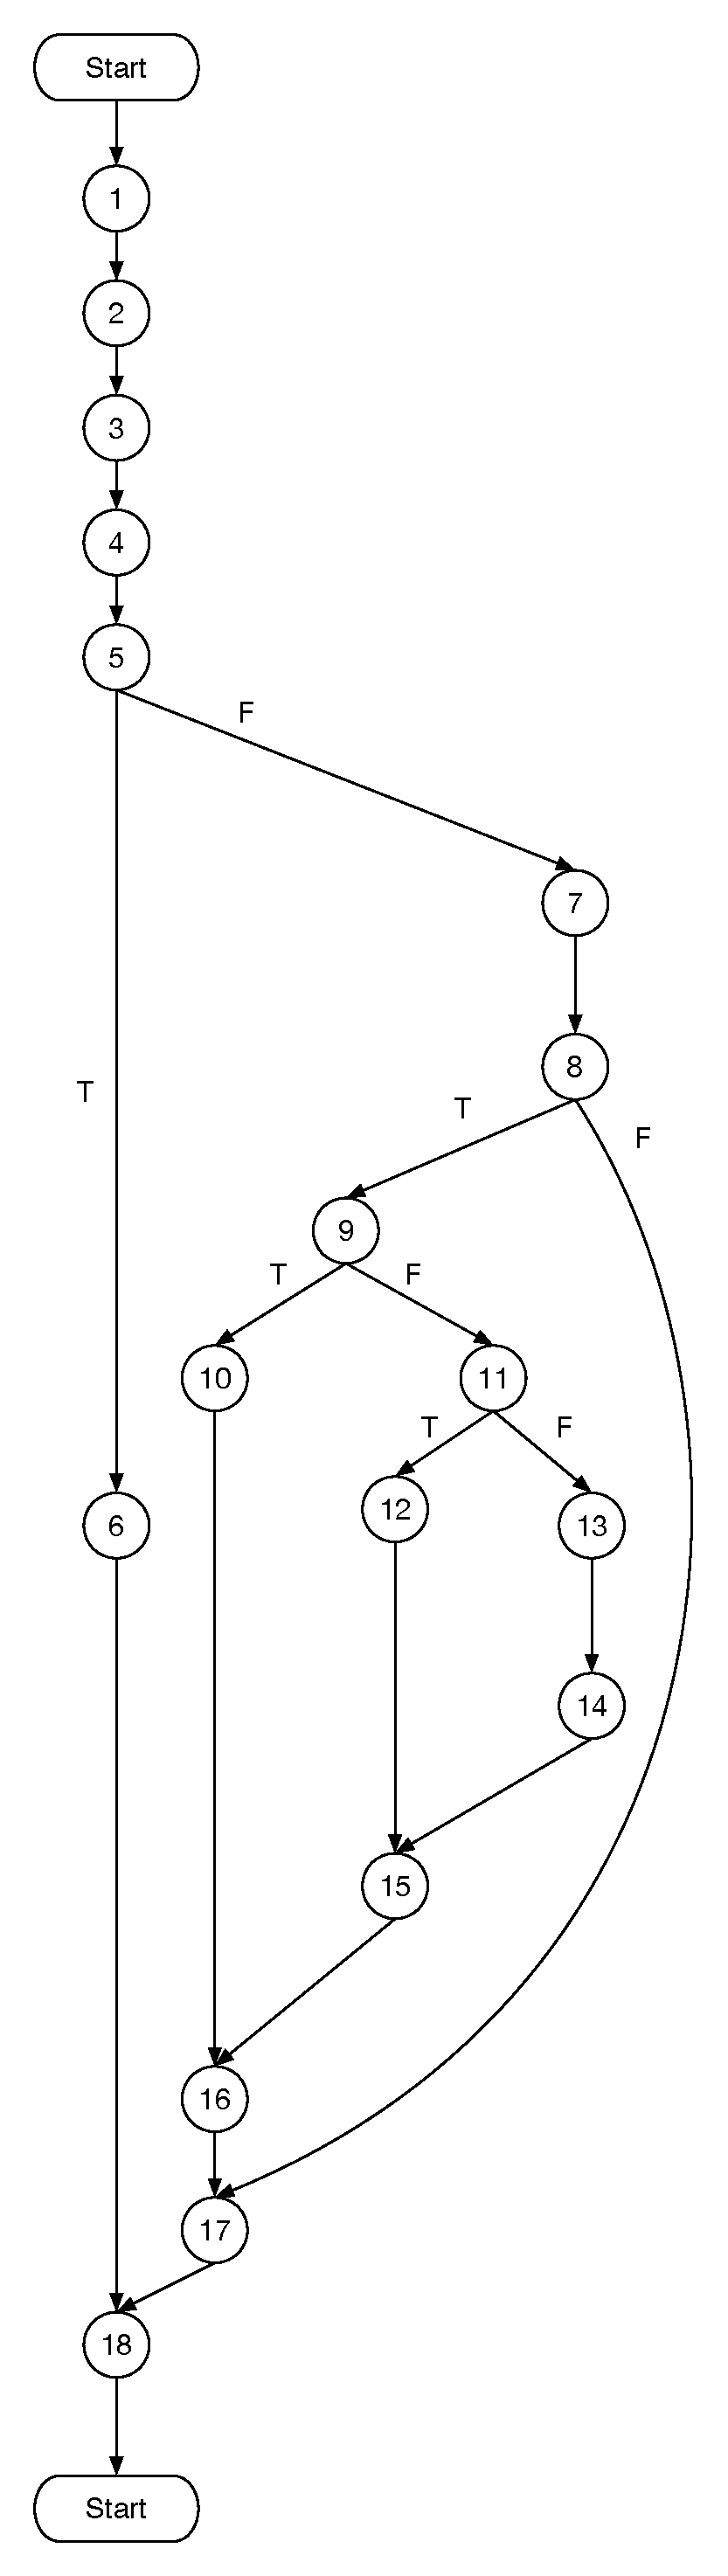
\includegraphics[height=0.8\textheight]{img/graph-testing.eps}
    \caption{Control flow graph ของโปรแกรมตรวจสอบรูปสามเหลี่ยมจาก \lstlistingname\, \ref{listing:trianglecal}}
\end{figure}

\newpage
\begin{landscape}
% Coverage table
    \section{Coverage table}

    \begin{table}[hb!]
        \caption{Coverage Table}
        \label{table:coveragetable}
        \begin{center}
            % ID, Path, Decisionx3, Inputx3, Expected output = 9 cols
            \begin{tabular}[p]{ | c | l | *{7}{c|} l |}
                \hline
                \multirow{2}{*}{ID} & \multicolumn{1}{c}{\multirow{2}{*}{Path}} & \multicolumn{4}{|c|}{Decision} & \multicolumn{3}{|c|}{Inputs} & \multicolumn{1}{c|}{\multirow{2}{*}{Expected Output}} \\ \cline{3-9}
                                    &                                           & 5 & 8 & 9 & 11 & a   & b   & c   &                \\ \hline
                1 & $1-2-3-4-5-6-18$                                            & T & - & - & -  & 201 & 201 & 201 & \outbound      \\ \hline
                2 & $1-2-3-4-\bar{5}-7-\bar{8}-17-18$                           & F & F & - & -  & 100 & 1   & 1   & \nottriangle   \\ \hline
                3 & $1-2-3-4-\bar{5}-7-8-9-10-16-17$                            & F & T & T & -  & 100 & 100 & 100 & \equ           \\ \hline
                4 & $1-2-3-4-\bar{5}-7-8-\bar{9}-11-12-15-16-17-18$             & F & T & F & T  &   3 &   4 &   5 & \sca           \\ \hline
                5 & $1-2-3-4-\bar{5}-7-8-\bar{9}-\bar{11}-13-14-15-16-17-18$    & F & T & F & F  & 100 & 100 &  50 & \iso           \\ \hline
            \end{tabular}
        \end{center}
    \end{table}
\end{landscape}
\end{document}
